% CAPITULO 1: EXPLICO EL ESQUEMA GENERAL DEL ALGORITMO
\chapter{Esquema general del algoritmo/método}

Desde un punto de vista abstracto, se puede pensar en el método como
En este caso, la función a optimizar está dada por el resultado de  .Una particularidad de este problema es que, 
si bien no conocemos su forma funcional ni podemos resolver el problema del su valor mínimo() 
tenemos cierta información acerca de la imágen de esta función, o al menos del valor al cual queremos llegar.
El uso de un método probabilistico apunta a mejorar la performance en la búsqueda de la solución pero también aporta propiedades no deterministas al algoritmo.

En la figura \ref{fig:esquema-algoritmo} se ve un esquema general del método, aplicado al problema de secuencias que queremos tratar. En esta sección se explicarán mas en detalle l

\begin{figure}[htbp]
\centering
   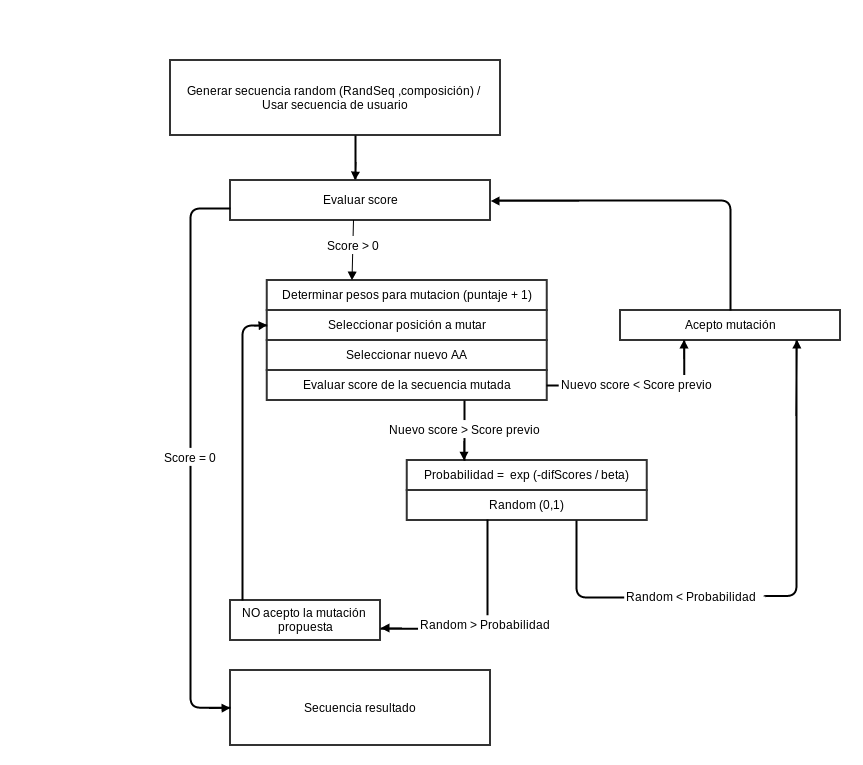
\includegraphics[width=\textwidth]{img/diagrama-algoritmo.png}
 \caption{Esquema general del método aplicado para obtener la secuencia final}
 \label{fig:esquema-algoritmo}
\end{figure}


\section{Secuencia inicial}

El algoritmo itera a partir de una secuencia inicial. 
Esta secuencia puede ser creada de forma aleatoria como primer paso del algoritmo o puede ser pasada por parámetro. 
% (mediante el parámetro --seq).

La generación de una secuencia aleatoria no es un problema trivial. 
En la naturaleza las proteínas están compuestas de un conjunto de 20 aminoácidos, los cuales se encuentran con diferentes abundancias relativas. 
La frecuencia de cada aminoácido dentro de un proteoma está dada por un balance entre el costo metabólico de este y la necesidad de contar con un conjunto de secuencias diversas que darán proteínas funcionales \cite{krick2014amino}. 
Para generar una secuencia aleatoria, entonces, es necesario definir la frecuencia que tendrá cada aminoácido. Esta frecuencia se obtiene a partir de la frecuencia global que tiene cada aminoácido en la base de datos de secuencias proteicas.
La aplicación que se utiliza para obtener la secuencia random es RandSeq 
HAY REFERENCIA PARA LA APLICACION?
(http://web.expasy.org/randseq/). Entre otras que existen, esta herramienta ofrece la posibilidad al usuario de definir las frecuencias que desea para cada aminoácido, o usar por default la composición estándar obtenida de SwissProt.  
Los valores de la composición estándar se encuentran en http://web.expasy.org/protscale/pscale/A.A.Swiss-Prot.html
Estos valores resultan del cálculo de la composición de aminoácidos de todas las proteínas de la base de datos. De esta forma, la composición total representa un consenso de frecuencias de aminoácidos entre todas las secuencias documentadas hasta el momento.

El programa permite también indicar solo la frecuencia de algunos residuos en particular, dejando el restos con la frecuencia estándar. INCLUIR EJEMPLO.
¿POR QUE LE SERVIRIA ESTO A UN DISEÑADOR DE PROTEINAS?
Esta funcionalidad permitiría, por ejemplo indicar que cierto aminoácido no esté presente en la secuencia (asignándole una frecuencia igual a 0). Para el fin que tiene la herramienta, es útil tener este tipo de funcionalidades ya que permite adaptar los requerimientos a las capacidades(limitaciones) del laboratorio experimental. El nuevo linker diseñado deberá poder ser sintetizado eficientemente junto con la nueva proteína, lo cual implica una carga metabólica para el sistema biológico en el cual está siendo producido. De esta forma, se intentará adaptar las propiedades de la secuencia diseñada para aumentar la capacidad de síntesis reduciendo, por ejemplo, los aminoácidos que implican un gran gasto energético y que limitarán la producción de la proteína final.


DESPUES INCLUIR SNAPSHOT DEL FORMULARIO


\section{Esquema de mutación}

El procedimiento general del algoritmo consiste en iterar sobre la secuencia inicial, evaluando en cada paso las propiedades de cada posición de la secuencia con respecto a características de interés. 
Los resultados de cada evaluación serán reflejados en un valor numérico o puntuación asociado a cada posición. En cada iteración el puntaje es inicializado en 0 para todas las posiciones y cada evaluación ejecutada puede aumentar o mantener el valor, de manera tal que, al finalizar todas las evaluaciones correspondientes a una iteración, el puntaje de cada posición tendrá un valor mayor o igual a cero. 
El aumento de este puntaje depende de la concordancia que tiene cada posición con las características evaluadas. En cada evaluación se aumenta el valor si el residuo en esa posición NO favorece la propiedad deseada.
Al terminar todas las evaluaciones de cada iteración, el puntaje resultante se utiliza para decidir si es necesario realizar una mutación sobre la secuencia y, de ser así, sobre que posición se realiza.
PONER EJEMPLO PARA QUE QUEDE CLARO

DIBUJAR DIAGRAMA DE FLUJO O PSEUDOCODIGO DEL ALGORITMO

El proceso de mutación se realiza al final de cada iteración y consta de dos pasos:
    -En primer lugar se selecciona uno de los residuos de la secuencia como objetivo para realizar la mutación. Esta selección será ponderada, utilizando como factor de ponderación el puntaje asociado a cada posición. Se debe tener en cuenta que, como se mencionó previamente, el valor del puntaje resultante puede ser igual a 0 y, si esto se repite para todas las posiciones, puede ocurrir que ningún residuo sea factible de ser seleccionado, en cuyo caso no se continúa el proceso de mutación. 
    -El segundo paso, asumiendo que algún residuo fue seleccionado, consiste en seleccionar con que aminoácido se sustituirá éste. Esta selección se realiza siguiendo la misma distribución que se utilizó para generar la secuencia inicial. Dado que la selección del sustituto es independiente del tipo de residuo seleccionado para mutar, es posible que el mutado y su reemplazo seleccionado sean iguales. En este caso simplemente se vuelve a seleccionar un sustituto hasta que el resultado sea un residuo distinto al anterior.     

    -El tercer paso consiste en aceptar o rechazar la mutación según un algoritmo de Monte Carlo. Para realizar esto se vuelve a evaluar el puntaje, analizando todas las características deseadas de la secuencia pero, esta vez, el análisis se hará sobre la secuencia que contiene la mutación propuesta, la cual se aceptará si el puntaje asociado es menor que el  resultante de la secuencia sin la mutación incorporada. De forma resumida, solo se incorporan mutaciones que se traduzcan en una disminución del puntaje total de la secuencia.
En caso de no aceptarse la mutación propuesta el algoritmo vuelve al primer paso del proceso de mutación.

El algoritmo busca, en cada iteración, reducir el puntaje de la secuencia introduciendo una mutación. Dado que el objetivo final es obtener una secuencia que posea, con cierta probabilidad, todas las características deseadas, el algoritmo finaliza cuando el puntaje resultante sea igual a cero. Esto implica que todas las evaluaciones concuerdan con los objetivos buscados en el diseño de la secuencia linker.

